% This file was created with tikzplotlib v0.10.1.
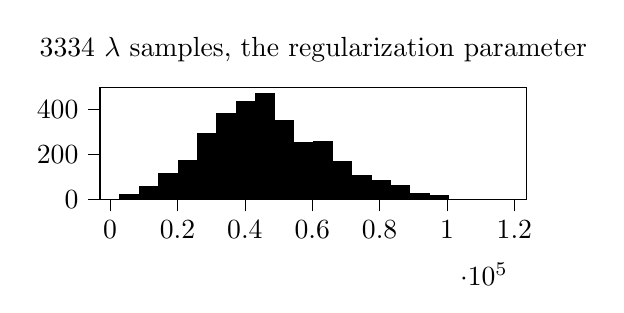
\begin{tikzpicture}

\definecolor{darkgray176}{RGB}{176,176,176}

\begin{axis}[
height=3cm,
tick align=outside,
tick pos=left,
title={3334 \(\displaystyle \lambda\) samples, the regularization parameter},
width=7cm,
x grid style={darkgray176},
xmin=-3012.30207843215, xmax=123641.428368197,
xtick style={color=black},
y grid style={darkgray176},
ymin=0, ymax=496.65,
ytick style={color=black}
]
\draw[draw=none,fill=black] (axis cs:2744.68566914189,0) rectangle (axis cs:8501.67341671592,25);
\draw[draw=none,fill=black] (axis cs:8501.67341671592,0) rectangle (axis cs:14258.66116429,62);
\draw[draw=none,fill=black] (axis cs:14258.66116429,0) rectangle (axis cs:20015.648911864,118);
\draw[draw=none,fill=black] (axis cs:20015.648911864,0) rectangle (axis cs:25772.636659438,175);
\draw[draw=none,fill=black] (axis cs:25772.636659438,0) rectangle (axis cs:31529.6244070121,296);
\draw[draw=none,fill=black] (axis cs:31529.6244070121,0) rectangle (axis cs:37286.6121545861,385);
\draw[draw=none,fill=black] (axis cs:37286.6121545861,0) rectangle (axis cs:43043.5999021601,440);
\draw[draw=none,fill=black] (axis cs:43043.5999021601,0) rectangle (axis cs:48800.5876497342,473);
\draw[draw=none,fill=black] (axis cs:48800.5876497342,0) rectangle (axis cs:54557.5753973082,356);
\draw[draw=none,fill=black] (axis cs:54557.5753973082,0) rectangle (axis cs:60314.5631448822,258);
\draw[draw=none,fill=black] (axis cs:60314.5631448822,0) rectangle (axis cs:66071.5508924563,259);
\draw[draw=none,fill=black] (axis cs:66071.5508924563,0) rectangle (axis cs:71828.5386400303,172);
\draw[draw=none,fill=black] (axis cs:71828.5386400303,0) rectangle (axis cs:77585.5263876043,107);
\draw[draw=none,fill=black] (axis cs:77585.5263876043,0) rectangle (axis cs:83342.5141351784,86);
\draw[draw=none,fill=black] (axis cs:83342.5141351784,0) rectangle (axis cs:89099.5018827524,64);
\draw[draw=none,fill=black] (axis cs:89099.5018827524,0) rectangle (axis cs:94856.4896303264,28);
\draw[draw=none,fill=black] (axis cs:94856.4896303264,0) rectangle (axis cs:100613.4773779,22);
\draw[draw=none,fill=black] (axis cs:100613.4773779,0) rectangle (axis cs:106370.465125474,3);
\draw[draw=none,fill=black] (axis cs:106370.465125474,0) rectangle (axis cs:112127.452873049,2);
\draw[draw=none,fill=black] (axis cs:112127.452873049,0) rectangle (axis cs:117884.440620623,3);
\end{axis}

\end{tikzpicture}
